% THIS IS SIGPROC-SP.TEX - VERSION 3.1
% WORKS WITH V3.2SP OF ACM_PROC_ARTICLE-SP.CLS
% APRIL 2009
%
% It is an example file showing how to use the 'acm_proc_article-sp.cls' V3.2SP
% LaTeX2e document class file for Conference Proceedings submissions.
% ----------------------------------------------------------------------------------------------------------------
% This .tex file (and associated .cls V3.2SP) *DOES NOT* produce:
%       1) The Permission Statement
%       2) The Conference (location) Info information
%       3) The Copyright Line with ACM data
%       4) Page numbering
% ---------------------------------------------------------------------------------------------------------------
% It is an example which *does* use the .bib file (from which the .bbl file
% is produced).
% REMEMBER HOWEVER: After having produced the .bbl file,
% and prior to final submission,
% you need to 'insert'  your .bbl file into your source .tex file so as to provide
% ONE 'self-contained' source file.
%
% Questions regarding SIGS should be sent to
% Adrienne Griscti ---> griscti@acm.org
%
% Questions/suggestions regarding the guidelines, .tex and .cls files, etc. to
% Gerald Murray ---> murray@hq.acm.org
%
% For tracking purposes - this is V3.1SP - APRIL 2009

\documentclass{acm_proc_article-sp}
%\usepackage{algorithm2e}
%\usepackage{algpseudocode}

%\newcommand{\commentSW}[1]{\textbf{SW --} \emph{#1} \textbf{-- SW}}


\begin{document}

\title{Extracting Spatial Information From Place Descriptions}
%\titlenote{(Does NOT produce the permission block, copyright information nor page numbering). For use with ACM\_PROC\_ARTICLE-SP.CLS. Supported by ACM.}}
%\subtitle{[Extended Abstract]
%\titlenote{A full version of this paper is available as
%\textit{Author's Guide to Preparing ACM SIG Proceedings Using
%\LaTeX$2_\epsilon$\ and BibTeX} at
%\texttt{www.acm.org/eaddress.htm}}}
%
% You need the command \numberofauthors to handle the 'placement
% and alignment' of the authors beneath the title.
%
% For aesthetic reasons, we recommend 'three authors at a time'
% i.e. three 'name/affiliation blocks' be placed beneath the title.
%
% NOTE: You are NOT restricted in how many 'rows' of
% "name/affiliations" may appear. We just ask that you restrict
% the number of 'columns' to three.
%
% Because of the available 'opening page real-estate'
% we ask you to refrain from putting more than six authors
% (two rows with three columns) beneath the article title.
% More than six makes the first-page appear very cluttered indeed.
%
% Use the \alignauthor commands to handle the names
% and affiliations for an 'aesthetic maximum' of six authors.
% Add names, affiliations, addresses for
% the seventh etc. author(s) as the argument for the
% \additionalauthors command.
% These 'additional authors' will be output/set for you
% without further effort on your part as the last section in
% the body of your article BEFORE References or any Appendices.

\numberofauthors{3} %  in this sample file, there are a *total*
% of EIGHT authors. SIX appear on the 'first-page' (for formatting
% reasons) and the remaining two appear in the \additionalauthors section.
%
\author{
% You can go ahead and credit any number of authors here,
% e.g. one 'row of three' or two rows (consisting of one row of three
% and a second row of one, two or three).
%
% The command \alignauthor (no curly braces needed) should
% precede each author name, affiliation/snail-mail address and
% e-mail address. Additionally, tag each line of
% affiliation/address with \affaddr, and tag the
% e-mail address with \email.
%
% 1st. author
\alignauthor
Arbaz Khan\\
       \affaddr{Department of Computer Science and Engineering}
       \affaddr{Indian Institute of Technology Kanpur}\\
       \affaddr{Uttar Pradesh, India}\\
       \email{arbazk@iitk.ac.in}
% 2nd. author
\alignauthor
Maria Vasardani\\
       \affaddr{Department of Infrastructure Engineering}\\
       \affaddr{University of Melbourne}\\
       \affaddr{Victoria, 3010}\\
       \email{mvasardani\\@unimelb.edu.au}
% 3rd. author
\alignauthor Stephan Winter\\
       \affaddr{Department of Infrastructure Engineering}\\
       \affaddr{University of Melbourne}\\
       \affaddr{Victoria, 3010}\\
       \email{winter@unimelb.edu.au}
}
% There's nothing stopping you putting the seventh, eighth, etc.
% author on the opening page (as the 'third row') but we ask,
% for aesthetic reasons that you place these 'additional authors'
% in the \additional authors block, viz.
% \additionalauthors{Additional authors: John Smith (The Th{\o}rv{\"a}ld Group,
% email: {\texttt{jsmith@affiliation.org}}) and Julius P.~Kumquat
%(The Kumquat Consortium, email: {\texttt{jpkumquat@consortium.net}}).}
\date{\today}
% Just remember to make sure that the TOTAL number of authors
% is the number that will appear on the first page PLUS the
% number that will appear in the \additionalauthors section.

\maketitle
\begin{abstract}
  A computational model of understanding place descriptions is a cardinal issue in multiple disciplines and provides critical applications especially in dialog-driven geolocation services. This research targets the automated extraction of spatial triplets to represent qualitative spatial relations between recognized places from natural language place descriptions via a simple class of locative expressions. We attempt to produce triplets, informative and \textit{convenient} enough as a medium to convert verbal descriptions to graph representations of places and their relationships. We present a reasoning approach devoid of any external resources (maps, path geometries or robotic vision) for understanding place descriptions. We then apply our methodologies to situated place descriptions and study the results, its errors and implied future research.
%We also provide an insight into the complexity of the untackled problem of resolving the frame of reference.
\end{abstract}

% A category with the (minimum) three required fields
\category{H.3.1}{Information Storage and Retrieval} content analysis and indexing - \textit{Linguistic processing} 
%A category including the fourth, optional field follows...
\category{I.2.7}{Artificial Intelligence}Natural Language Processing - \textit{Language parsing and understanding}

\terms{Experimentation, algorithms, languages, performance}

\keywords{Place descriptions, spatial role labelling, spatial language understanding, locative expressions, triplets} % NOT required for Proceedings

\section{Introduction}
A place description provides spatial information in terms of spatial features and the spatial relations between them. Place descriptions are used in everyday activities in spatial learning, problem solving and decision support in large-scale environments, independent and typically in absence of access to a map or a compass. The task of mapping a two-dimensional environment into a linear structure of language descriptions can also take a dynamic nature where a human uses a tour route for communicating spatial information \cite{linde:spatial, daniel:modes}. Thus, place descriptions can also be thought of encompassing path descriptions. To add to the complexity, the spatial features in the descriptions can be simple spatial features (house, park) or place names (official or informal). Nonetheless, this challenging task of understanding the natural language place descriptions provides critical applications in numerous domains including instruction following robots, description based localization in query/dialog based navigation services and automated geo-tagging of text. Also, having inferred the spatial relations from such a description, the translation of the relatively abstract verbal descriptions to more iconic media of conveying information (e.g., pictures and sketch maps) becomes easier.

This research targets the automated extraction of spatial triplets to represent spatial features and relations between them from natural language place descriptions via a degenerate form of locative expressions. \textit{Locative expressions} as described by Herskovits \cite{herskovits:pragmatics}, are expressions containing a preposition, its object and whatever the prepositional phrase modifies (i.e., subject of preposition). We, however, start from a degenerate form of locative expressions that are devoid of a subject. We provide a detailed definition for such expressions in Section \ref{DLE}. The challenge of this paper is to extract the subject of the DLEs to complete a spatial triplet.
%However, we area \textit{Degenerate Locative Expression} (DLE) can be described as an expression containing a preposition and its object, or simply a noun place (no prepositions).

The extraction process is accompanied with a trained learning model (\cite{fei:locative}) which predicts the beginning and the span of a degenerate locative expression in a sentence using Conditional Random Fields (CRFs) along-with the place names indicators (gazetteers and manual annotations). It gives a good indication on the spatial relations in Natural Language (NL) text and can be used to extract triplets in the format of an object of interest, a reference object and a prepositional relation that connects the two . This representation is derived from the technique of Spatial Role Labelling (SpRL) \cite{Kordjamshidi:labelling}, where the preposition serves as a spatial indicator connecting a trajector (object of interest) with a landmark (reference object). The end goal of this effort is to ease the translation of verbal descriptions to graph representations (with features as nodes and relations as edges). The aim is to make the triplets as \textit{informative} and \textit{convenient} as possible for such a translation. By being \textit{informative}, we mean to exploit the spatial information in the three components of the triplets. Also, the triplet output format becomes \textit{convenient} enough to a translator if it cuts down the linguistic complexities.

%A spatial frame of reference conceptualizes spatial cognition. Describing the location of an object can be broadly classified into two categories - egocentric and allocentric
The introduction of the problem leads to the fundamental question: Given a degenerate locative expression, is it possible to extract the spatial triplets without introducing any additional ambiguities? If yes, how effective is it to use degenerate locative expressions (DLEs) to identify the underlying spatial relationships between the places. In this paper we present a technique to identify the spatial relationships between recognized objects and place names with the help of DLEs. We claim our identified spatial relations to be qualitative and informative enough to assist in sketch-map generation and graphical depictions. However for the purpose of extraction of triplets, we are targeting only the static relations in the descriptions. We then investigate the different types of errors in the results of triplet extraction and highlight the gaps in the approach of its inability to resolve the indirect reference in a description and end by pointing out the challenges for dealing with full-blown English place descriptions.
%The proposed technique aims to handle the static nature of place descriptions.
%We also discuss the results of our technique and its quality as compared to the previous machine-learning approaches to the problem. Finally, we end by providing concluding remarks on our work and the future research implied by it.
\section{Relevant Work}
We are interested in the extraction of geographic information in the form of triplets, from unrestricted NL place descriptions. Research in the past had focused on mining specific and application-dependent geographic information from controlled language expressions \cite{kelleher:perceptually, Hanjing:route, tappan:knowledge} or from certain contexts, such as route descriptions. Linguistic constructs are often complex and lead to under or over-specifications when trying to match NL to formal frameworks of spatial information. As argued in \cite{Bateman:ontology}, most computational aspects of geographic information do not consider these linguistic intricacies, especially in the construction of formal models of spatial relations based on the logic of human spatial cognition. The authors also argue that such formal models do not acknowledge the way that people actually express spatial relations linguistically. Therefore, Bateman \cite{Bateman:language} suggests a semantics and linguistics based spatial ontology that would facilitate better mappings between spatial calculi and NL spatial expressions, such as the Generalized Upper Model ontology (GUM) \cite{Bateman:data}.

In more recent works, researchers have been working on parsers that can process unrestricted language input, and thus, come closer to the parser discussed in this paper. For example, Zlatev \cite{zlatev:semantics} worked on the cognitive linguistic research in spatial semantics and provided basic theoretical concepts for understanding it, in the form of the holistic spatial semantic theory. Based on that theory, Kordkamshidi et al. \cite{kordjamshidi:language} then implemented spatial role labeling (SpRL), a method with which they assigned reference objects, locata and spatial relations roles to linguistic terms. This technique facilitates mapping the terms onto formal spatial relations and is also used in this work. The authors suggest machine learning techniques to deal with ambiguity in linguistic spatial information and in \cite{Kordjamshidi:labelling}, they utilize the proposition project (TPP) from SemEval-2007 \cite{litkowski:semeval} for disambiguating the spatial meanings of prepositions and enhancing the SpRL technique.
Zlatev \cite{zlatev:semantics} worked on the cognitive linguistic research in spatial semantics and provided basic theoretical concepts for understanding it. Ever since then, there has been growing trend to understand natural language (NL) descriptions. The research has moved towards understanding unrestricted NL in current works (\cite{Kordjamshidi:labelling, matuszek:following, tellex:language}).
%Understanding natural language instructions in robotics and inferring paths using the knowledge of maps and %path geometries has been successfully dealt with \cite{kollar:robotic}, but the work on grounding spatial motion using the formal study of linguistics and spatial cognition %(and no external resources) is still in its early stages.
%
%Mani et. al \cite{mani:motion} provide the theoretical linguistic study on expression of motion. Kolomiyets et. al \cite{kolomiyets:semeval} have provided an annotation %scheme and the annotated dataset to study motion detection in NL text. This dataset was employed by Bastianelli et. al \cite{bastianelli:unitor} to address the task of %identifying spatial roles but the results indicate a weaker performance in a situated description comprising complex text. Most of these works make use of map-assisted %learning and/or vision based understanding (\cite{kollar:robotic,levit:interpretation,macmahon:walk}).
The methodology suggested in this paper makes use of no external resources (such as maps, vision), but employs a machine learning tool \cite{fei:locative} to identify place names and the associated prepositional phrases. Hereafter, we work with the concept and reasoning approach to form rules for extracting useful spatial information from the text.
\section{Theory}
\subsection{Definitions}
In this section, comprehensive definitions of the major terms that appear in this paper, viz spatial triplets (or simply triplets) and degenerate locative expressions (DLE), are provided.
\subsubsection{Spatial Triplets}
A spatial triplet is a triple of a locatum (\textit{LOC}), reference object (\textit{RO}) and a spatial relation (\textit{r}). Here, RO is the object by which the location of the LOC is defined, using the prepositional relation \textit{r}. For example, \texttt{<Melbourne Hospital $diagonally$ $across$ Peter Doherty Institute>} references \textit{Melbourne Hospital} as the LOC in terms of \textit{Peter Doherty Institute} as RO by the relation \textit{diagonally across} as \textit{r}. Vasardani et al. \cite{maria:descriptions} provide more information on the theory and the structure of triplets. This method of defining spatial relation is derived from the technique of Spatial Role Labelling(SpRL), which first appeared in \cite{Kordjamshidi:labelling}. In SpRL, one assigns spatial role labels to the words or phrases in sentences from the set \{\textit{trajector} (tr), \textit{spatial Indicator}(si), \textit{landmark}(l), \textit{none}\}. For example, such a labelled sentence looks like:
``[\textit{We}]$_{tr}$ are sitting [\textit{in}]$_{si}$ [\textit{the Baretto's}]$_l$ [\textit{in}]$_{si}$ [\textit{the Alan Gilbert Building}]$_{l}$''. However, spatial triplets that could be extracted out of such a sentence look like : \\<\texttt{We ${in}$ the Baretto's}> \\<\texttt{We ${in}$ the Alan Gilbert Building}>\\
Arguably, a spatial triplet relation provides a more convenient representation of spatial information than the role labels, and provides a suitable medium to translate the verbal description to a graph representation.
\subsubsection{Degenerate Locative Expressions (DLE)}
\label{DLE}
%In mathematics, a degenerate case is a limiting case in which a class of object changes its nature so as to belong to another, usually simpler, class
A locative expression is a spatial referring expression which contains a preposition, its object, and whatever the prepositional phrase modifies (i.e., subject of preposition) \cite{herskovits:pragmatics}. These expressions have been adopted as a standard for spatial semantics and cognition and are widely referred to \cite{olivier:semantics,zlatev:semantics}. However, in informal communication or a situated dialog, people tend to disregard the subject and describe the location in terms of just the preposition and its object (e.g., [I am] at Deakin University). We term such locative expressions as degenerate locative expresssions (DLE). In a crowdsourced corpus of place descriptions\footnote{Data collected by a mobile location-based game, \texttt{http://telluswhere.net/}} people described their location mostly in terms of DLEs (e.g., \textit{at the University of Melbourne}, \textit{in my house}). Hence, an attempt was made to identify the DLEs and train a model on this available dataset to provide predictions on any test corpus.
\newpage
\subsubsection*{Classification of Degenerate Locative Expressions}
From the definition of a degenerate locative expression (DLE), one can think of constructions like ``of the train-station'', ``from the University'' and ``to Bourke Street''. Such examples do follow from the definition but cannot convey any spatial relationship independently. Binary spatial relationships are not informative when naively using non-locative prepositions (e.g., X \textit{from} Y is not an informative relationship). Such DLEs require special treatment before the corresponding triplet relation could be extracted. We term such DLEs as \textit{partial DLE}s. These expressions include all those spatial expressions which do not start with locative prepositions\footnote{Here we don't deal with the exhaustive list of locative prepositions (Jackendoff and Landau \cite{landau:and}) but focus only on \textit{at, in} and \textit{on} as locative prepositions, the rest of the prepositions are treated as non-locative.}.
The rest of the DLEs, which start with a preposition of location and thus give a sense of spatial relation are termed as \textit{locative DLE}s. For example, \textit{in the alley} is a locative DLE. The procedures for triplet extraction described in the subsequent sections are described first for locative DLEs and then for partial DLEs.
%Some partial DLEs can be converted to locative DLEs by completing the prepositional clause to form a locative phrase (e.g. ``from the University" can complete to ``at the 3rd house from the University" and ``of the train-staion" to ``in the north of train-station"). Such DLEs are converted so and thenceforth handled like locative DLEs.
%Example for verb: I am living 2 blocks away from the station
%Example for adjective: my house is next to the station.
\subsection{Extracting Spatial Triplets}
To deal with the task of spatial information extraction, we set ourselves the aim of identifying `informative' triplets. The problem can be defined similar to a spatial role labelling task (SpRL), the difference being that we attempt not to miss any information from the place names and the spatial relation. For an example from the SpRL dataset, ``two men are standing on a lawn in front of a light brown house with blue corners'', SpRL marks one of the reference object as `house' to eventually give the triplet \texttt{<lawn $in$ $front$ $of$  house>}. However, we are interested in including any informative meaning inherent in the description and thus output ``lawn in front of light brown house''. This also becomes essential in the long term goal of translating verbal descriptions to graphical depictions, where the graph/sketch drawing algorithm could be vitally benefitted by localizing the spatial feature to `light brown house' rather than just any `house' (from the above example). There have been various datasets used for identifying spatial expressions \cite{Bateman:data,CLEF:data, parisa:semeval}  but none are characteristic enough of a place description. For instance, place descriptions are more descriptive than mere spatial expressions and the spatial relations can be fairly complex and difficult to formalise (e.g., `between', `across from').  Due to the goals set thereafter and the fact that there is no available dataset for training on such special and essential requirements, a reasoning approach, rather than a machine-learning approach is chosen here for extracting triplet relations. This approach helps in understanding place descriptions and thus eventually aiding machine learners by revealing the structure and identifying relevant/irrelevant attributes.
%in identifying the better features and deciding the distribution of weights to these features.

Extracting triplet relations poses varying challenges owing to the complex nature of place descriptions. The spatial relations can be defined either simply using position descriptors (e.g., on, at, in) or using concepts of motion and indirect references \cite{zlatev:semantics}. For example, in ``From here, you can go left towads X and then head north to reach Y'', the phrase ``from here'' carries context (indirect reference) and the current context is shown spatially related to X and Y via motion indicators. For the purpose of this paper we limit ourselves from the detection of spatial motion and resolution of indirect references and instead focus on the structure of static place-descriptions. The triplet extraction assumes all descriptions are static, i.e., without any context or motion. This process of extraction of triplets goes through the DLEs by categorising them into the two types: \textit{locative} and \textit{partial}. We start by describing the process of triplet extraction for locative DLEs, and then move forward to deal with partial DLEs.
\subsubsection*{Locative DLEs}
Given the DLEs, to identify the triplet relation, one needs to find the subject of DLE. For example, in ``There is a construction site in the alley'', the DLE is `in the alley' and the triplet relation extracted should be \texttt{<construction site $in$ the alley>}. To  identify the subject, the dependency between the preposition \textit{in} and the two noun places `construction site' and `the alley' need to be identified. Luckily, from the Stanford typed dependencies parser \cite{marneffe:stanford} one can extract the dependencies between the words of a sentence. Using the collapsed dependencies representation, \textit{prep} relation reports a prepositional phrase and the verb/noun/adjective modified by the prepositional phrase. In the syntactic terminology of the Stanford dependency parser, the former is called the dependent and the latter is called the governor. In this case, the dependency reported is \textit{prep\_in}(site,alley) where `site' is the governor and `alley' is the dependent. When the relation is between two nouns, the triplet relation is direct.
%\footnote{A noun place can also be a nominal subject to a noun. For e.g, in "AGB is the first building on the Grattan Street", the dependency is prep\_\textit{on}(building, Street) and nominal subject of "building" is AGB. Hence AGB is reported as the subject.}
However, in the case of verb/adjective, we further explore the typed dependencies to find the subject or the noun modified by the corresponding verb/adjective. The subject finding task (for verb/adjective/noun) then recursively checks for the modifiers of the subject (if any) by searching through the set of modifier relations provided by typed dependencies. The final triplet relation is reported thereafter. The steps to extract triplets from a sample sentence for the case of \textit{prep} relation involving a verb is shown in Figure~\ref{fig:phase1}.

In descriptions where a person describes a location using references to pronouns, e.g., \textit{You can also find NAB and Commonwealth bank branches near the Union House}, the direct object of the verb gets linked to its prepositional relation (\textit{near}). So, in this sentence, subject of the verb \textit{find} is \textit{You}, but the direct objects are \textit{NAB} and \textit{Commonwealth Bank}, and thus the triplet should be \texttt{<NAB $near$ Union House>} (and not \textit{You near Union House}). Thus, the heuristic that works here is: if there is a direct object of the verb, report the direct object as the locatum of the triplet. The heuristic can be further strengthened by using the fact that in such cases the nominal subject of the verb is a pronoun.
\begin{figure}
\centering
%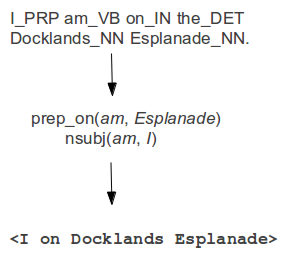
\includegraphics[width=0.5\textwidth]{phase1.png}
\epsfig{file=phase1.eps, height=2.3in, width=1.7in}
\caption{Sample run of the identification process for locative DLE in the sentence  ``I am on the Docklands Esplanade''}
\label{fig:phase1}
\end{figure}
\begin{table*}
\centering
\caption{Extending the prepositional relations of direction using Stanford dependencies (DEP)}
\begin{tabular}{|c|c|p{4cm}|p{5cm}|} \hline
\textbf{Governor}&\textbf{Action on relation}&\multicolumn{2}{|c|}{\textbf{Example}} \\ \cline{3-4}
&&\textbf{Sentence}&\textbf{Actions}\\ \hline
noun & extend with the noun and its modifiers&Its the 3rd house from the station.&DEP : \textbf{prep\_from}(house, station) \\&&&extends \textit{from} to ``3rd house from'' \\ \hline
adjective & extend with the adjective&My house is next to the station.&DEP : {\textbf{prep\_to}}(next, station) \\&&& extends \textit{to} to ``next to''\\ \hline
verb & extend with the verb's modifiers*&I am living 2 minutes from the station.&DEP : \textbf{prep\_from}(living, station)\\&&& adds modifiers of \textit{living} (`2 minutes')\\&&& extends \textit{from} to ``2 minutes from''\\
\hline\end{tabular}
\\ \begin{flushleft}
*-preference to verb's direct object (if any)
\end{flushleft}
\label{table:partial}
\end{table*}
\subsubsection*{Partial DLEs}
The partial DLEs convey no spatial information independently but they form a medium for inferring spatial relationships in the place description. As mentioned earlier, partial DLEs can be converted to locative DLEs in some sentences and can be directly used to output triplets. In other cases, a partial DLE can be made informative and meaningful by just extending its prepositional clause. For example, consider the sentence ``I am 300 meters far from the auburn train-station'' with the partial DLE ``from the auburn train-station''. Clearly, by including the ``300 meters far [from]'' we get a more informative triplet \texttt{<I 300 $meters$ $far$ $from$ the train station>}. Thus, the aim is to capture this information from the typed dependencies. Table \ref{table:partial} provides the exhaustive rules to extract this information from the typed dependencies. By doing this, we exploit the locative purpose served by a partial DLE. Thereafter, we proceed similar to a locative DLE to find subject of the preposition.

%However, it should be noted that a directional DLE may not have a locative purpose at all. Instead, it may be specifically used to dynamically describe the spatial relations. For example, in "If you walk south from the engineering departments, you reach to the main south entrance", we see the implied spatial relationship of 'main south entrance' to be at the \textit{south} of 'engineering departments'. So, we keep such DLEs in the Phase-1 triplets even though no spatial information is conveyed. In Phase-II, such triplets are further processed to derive the implied spatial relationships.
%\subsubsection{Phase-II}
%After producing the triplets in Phase-I, we move to Phase-II where we process triplets carrying dynamic spatial relationships. Kuipers \cite{kuipers:modeling} argues the cognitive map of humans and the spatial knowledge as a catalog of routes and thus, supports the evidence for human place descriptions to possess a dynamic nature and contain an underlying tour route to the subject environment.


%\centerline{$\downarrow$ {\small (include modifiers)} \\}
%\newtheorem{algorithm}{Algorithm}
%\begin{algorithm}
%\While{$current\_position$ is inside circle,}{}
%Extract triplet relations from stanford collapsed dependencies \\
%\end{algorithm}

%But the preposition dependency is reported only in terms of phrase heads. As for this case, the dependency reported is \textit{prep\_in}(site,alley). Henceforth, to complete %the triplet relation with the help of dependencies, we include all the modifiers for the arguments of the dependency.

%~ \subsection{Understanding the complexity of frame of reference recognition}
%~ The set-up of the above methodology provides valid spatial relations only when the description contains a fixed frame of reference. However, the use of different frames of references in describing a place results in indirect references of a place. These indirect place references need to be resolved to be able to examine spatial relationships.
 %~ To understand the complexity of the problem, we used an annotation scheme on the actual spatial triplets expected from the available set of place descriptions. An extra field was added in the triplets data containing a sentence\_id which denotes counter index of the sentence in which a triplet is found. This helped in understanding the depth of the connections between the sentences. If a phrase of the triplet occurs as RO in a number of sentences, then we know how far the reference gets carried. The results and inferences of the study are summarised under Section \ref{sec:experimentalstudy}.

\section{Implementation}
The methodology mentioned in the previous section works on the natural language via the results of a parser which is trained to identify degenerate locative expressions in informal text \cite{fei:locative}. The parser builds a \textit{conditional random field} (CRF) machine learning model on the manually annotated corpus of place descriptions \cite{tuw} and attempts to identify both informal and formal place references. To enhance its prediction scores, it exploits external resources such as gazetteers and dictionaries. The output provided by the parser is in the form of IOB encoding as marked in Figure~\ref{fig:IOB}. A B-NP tag denotes the \textit{beginning} of DLE, while I-NP tags indicate the word is \textit{in} the span of a DLE. All words with O tags are \textit{outside} of any DLE. Hence, in the example shown in Figure~\ref{fig:IOB},  ``in Baretto'' and ``in Alan Gilbert Building'' are identified as DLEs in the sentence. The DLEs output by the parser are either simply place names (e.g., Chetwynd Place) or place names with prepositional attachments (e.g., of the train station).

The parser is written in \textit{Python} and our program works on top of it. The input requirements for the parser are met by \textit{Part-of-Speech} (POS) tagging and shallow parsing (\textit{chunking}) the sentences. POS-tagging corresponds to determining the part-of-speech tag (e.g., noun, verb, adverb) associated with a word, whereas shallow parsing is the process of grouping words in a sentence as \textit{chunks} to analyse the syntactic structures. Besides this, the parser can be aided in locating place references by marking the place names and manually annotating them with information such as granularity and identifiability. The format of these manual annotations follows the scheme provided by Tytyk and Baldwin \cite{igor:annotations}. The manual annotations are optional, but can be included to enhance the DLE prediction scores. For each DLE extracted from the parser, our program identifies its subject (after extending prepositional clauses for partial DLEs) using the output of the \textit{Stanford parser} \cite{klein:accurate} for POS tags and dependencies in the original sentences.
\begin{figure}
\centering
%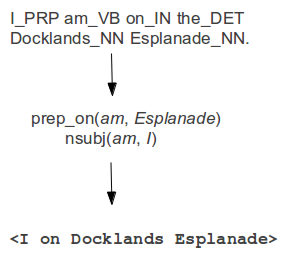
\includegraphics[width=0.5\textwidth]{phase1.png}
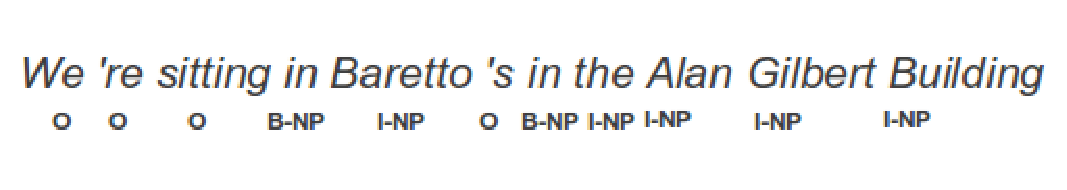
\epsfig{file=IOB.eps, height=0.53in, width=3in}
\caption{IOB-encoded identification of degenerate locative expressions}
\label{fig:IOB}
\end{figure}
%\[\textit{We're sitting} \underbrace{\textit{in Baretto's}} \underbrace{\textit{in the Alan Gilbert Building}}\]
\section{Experimental Study}
\label{sec:experimentalstudy}
In this section, the experimental analysis of our methodology is presented. First, the dataset used for testing out methodology is described. Next, an insight to the performance of our approach for extracting triplets from our corpora, the \textit{Tell Us Where} mobile game dataset and the set of campus descriptions, is given.  Finally, the errors produced in extracting the triplets and the sources behind them, as well as the types of triplets missed by the approach are discussed.
\newpage
\subsection{Dataset Description}
For our experimental study, we used the \textit{Tell Us Where} dataset \cite{tuw} as one of the test corpora. The dataset comes from a location based mobile game which locates its users and asks them: ``Tell us where you are''. Originally, the corpus consisted of 1,858 place descriptions but for the purpose of this research, descriptions containing fewer than 20 words are filtered out. This gives 54 distinct situated place descriptions, each of which describes relationships among two or more places. Additionally, a set of four NL descriptions of the Parkville campus of the University of Melbourne is parsed, none of which originally are less than 100 words. These were submitted by graduate students with varying degrees of familiarity with the campus. Also, there were no instructions given to the students while submitting the descriptions, which yields a set of unrestricted NL place descriptions. With such datasets, our testing model is set up to be descriptive enough, constraint-free and thus more natural in relation to, and characteristic of place descriptions. 
\subsection{Extraction Of Triplets}
\label{extraction}
The task of extracting `spatially informative' triplets from NL descriptions is challenging and cannot be directly dealt using simply a language parser. The DLE parser aids in separating the place names, and manual annotations to enhance the DLE parser are employed\footnote{The results do not differ considerably with the set-up of not using the manual annotations except for the errors described in \ref{subsub:DLE}}. This subsection focusses on the triplets extraction study pertaining to static place descriptions. The parser's output in such cases has a fair similarity with the expected triplets. Below are some of the example cases representative of the results.
\newtheorem{example}{Example}
\begin{example}
I am $[$at a 3 stories town house$]$, number 7 $[$Chetwynd Place$]$. $[$The house$]$ is located $[$in a small alley$]$ $[$behind a row of town house$]$ $[$along Chetwynd Street$]$, $[$near the corner$]$ $[$between Chetwynd Street and Queensberry Street$]$. There is $[$a construction site$]$ $[$in the alley$]$. Its the 3rd house from the head $[$of the alley$]$.
\end{example}
This example is taken from the \textit{Tell Us Where} corpus. The bracketed texts correspond to the DLEs identified by the parser. The triplets output by the program are presented in Table~\ref{table:ex1}. This is a characteristic example of a static place description without any indirect reference, except in the last sentence where `it' is used in place of ``the house'' and thus no triplet was extracted. If the sentence is rephrased as ``\textit{I am in the 3rd house from the head of the alley}'', the triplet extracted is, \texttt{<I $in$ $3rd$ $house$ $from$ the head of the alley>}\footnote{See how the preposition `from' gets extended to `3rd house from', and the clause related to the preposition `of' gets attached into the reference object as `head of the alley'}. Not all triplets inherent in the description were extracted (see Section~\ref{missing}). Nonetheless, from the output of the parser, the triplets produced seem promising and interpretable for an algorithm for graphical depiction.

The `between' relation in the example is spatially informative, but not syntactically suitable for a triplet, as it has two reference objects connected to the same locatum. This inhibits the computational interpretation of triplets. Vasardani et al. \cite{maria:descriptions} discuss the semantics of triplet relations, and propose that triples with `between' relation can be broken into two, by identifying the conjuncts of the dependent (here, `Chetwynd Street' and `Queensberry Street'). However, the conjuncts were not separately identified in this case because of the presence of the connector `and', which forces the DLE parser to identify \textit{Chetwynd Street and Queensberry Street} as one single place name, thus leading to a bias in the subject finding methodology. In a different case, where such a restriction does not hold because the word `the' follows a connector `and', triplets produced for a \textit{between} relation are shown below (Example \ref{ex:between}). The output comes out as suggested in \cite{maria:descriptions}.
\begin{example}
\label{ex:between}
Between this building and $[$the campus$]$, $[$on Swanston St$]$, is the major public transport hub for $[$the University $]$.
\end{example}
Triplets extracted:\\
\texttt{<the major public transport hub $between$  building>} \\
\texttt{<the major public transport hub $between$  the campus>} \\
\texttt{<the major public transport hub $on$ Swanston St>}
\begin{table}
\begin{tabular}{|l|}
\hline
\texttt{<I $at$ a 3 stories town house>}  \\ \hline
%Chetwynd Place \\ \hline
\texttt{<The house $in$ a small alley>} \\ \hline
\texttt{<a small alley $behind$ a row of town house>}\\ \hline
\texttt{<The house $along$ Chetwynd Street>}\\ \hline
\texttt{<The house $near$ the corner>}\\ \hline
\texttt{<the corner $between$ Chetwynd Street} \\
\texttt{and Queensberry Street>}\\ \hline
%\texttt{a construction site}\\ \hline
\texttt{<a construction site $in$ the alley}\\ \hline
%\texttt{<the head of the alley>}\\ \hline
\end{tabular}
\caption{Parser output for spatial triplet relations in Example 1}
\label{table:ex1}
\end{table}
\begin{example}
\label{ex:c1}
We're sitting $[$in Baretto$]$'s $[$in the Alan Gilbert Building$]$, $[$across Grattan street$]$ is one of the $[$ medical buildings $]$. $[$Down the hill$]$ $[$along Grattan street$]$ the $[$new building$]$ being constructed is the $[$Peter Doherty Institute$]$ and diagonally across the road ($[$Royal Parade$]$) is $[$Melbourne Hospital$]$. In the other direction the open area is $[$University square$]$ (there is a $[$carpark$]$ underneath). At the city end $[$of University square$]$ is $[$the law building$]$. $[$Across Grattan street$]$ $[$from University square$]$ there is $[$an entrance$]$ $[$to the campus$]$, straight ahead is $[$an overpass building$]$ and to the right are the various $[$Engineering buildings$]$. The road goes in a big loop around $[$the campus$]$ you can either go left $[$towards the Medical buildings$]$ or right passed $[$the Engineering buildings$]$ then head North (away from University square). One other area you may want to explore is $[$South Lawn$]$ which you can get to by going $[$underneath the overpass building$]$ directly in front of you when you enter $[$the campus$]$.
\end{example}
This is an example taken from the set of campus descriptions. The triplets output by the program are shown in Table~\ref{table:ex2}\footnote{The first and the third sentence were split at clause boundaries to eliminate Stanford parser errors; see Section~\ref{subsub:stanford}}. We observe that the static spatial relations come up as desired. For instance, the program infers the complex triplet relation:

\texttt{<an entrance \textit{across} Grattan Street}\\ \texttt{\textit{from} University Square>}
\begin{table}
\begin{tabular}{|l|}
\hline
\texttt{<We $in$ Baretto>}\\ \hline
\texttt{<We $in$  Alan Gilbert Building>}\\ \hline
\texttt{<one of medical buildings $across$ Grattan street>}\\ \hline
\texttt{<the Peter Doherty Institute $Down$ the hill>}\\ \hline
\texttt{<the hill $along$ Grattan street>}\\ \hline
\texttt{<the law building $at$  $the$ $city$ $end$ $of$ }\\
\texttt{University square>}\\ \hline
\texttt{<an entrance $across$  Grattan street} \\
\texttt{from University square>}\\ \hline
\end{tabular}
\caption{Program output for spatial triplet relations in Example 2}
\label{table:ex2}
\end{table}
with its complete inherent information using the DLEs related to it, i.e., $[$Across Grattan street$]$, $[$from University square$]$ and $[$an entrance$]$. Again for formalising reasons, the `across from' relation can be broken analogously to a `between' relation in the previous example. It can be seen, however, that not all triplets were extracted by the program because of issues such as indirect references in the phrases ``\textit{straight ahead \dots Engineering buildings}'' and ``\textit{In the other direction} \dots'', and spatial motion in the sentence, ``\textit{The road goes} \dots'', which are not dealt with currently by the parser.
\subsection{Investigating Errors}
From the results obtained by the test corpora, there was a clear indication that the validity of the produced triplets relies on the correctness of the Stanford typed dependencies, as well as the accuracy of the DLE parser. Some invalid cases are also the product of the subject finding methodology for the DLEs, mainly due to its inability to disambiguate the spatial sense in the subject. In other cases, it is the informal or incorrect usage of grammar that led to the failure of triplet extraction. Each of these cases are discussed in detail below.
\subsubsection{Invalid Subjects}
The errors corresponding to invalid subjects found can be prominently classified into two types: \textit{invalid place name} and \textit{subjects with unwanted information}. Since there is no spatial sense disambiguation done for the noun phrases, some of the subjects reported turn out to be invalid. For instance, in example \ref{ex:halfway}, the subject of the DLE \textit{along the street} is \textit{approximately halfway} (a noun phrase) and is deemed correct by the program, producing an incorrect triplet. Similarly in example \ref{ex:roses}, subject of \textit{at the gate and the house} is identified as \textit{roses} (instead of \textit{an arch}), which is not a place reference and thus is invalid. Such errors can be corrected by choosing subjects, which are identified as place references by the DLE parser. However, this leads to the side-effect of making the production of triplets heavily dependent on the accuracy of DLE parser.

Additionally, this approach of finding the subject of a DLE in the most informative way leads sometimes to extensions with undesired information. In the example \ref{ex:wilson}, \textit{Wilson Hall} gets undesirably extended to \textit{Wilson Hall a multi-function hall}, due to having DLEs separated by a comma identified as a single expression. While in most cases this rule provides useful spatial information (e.g., the University of Melbourne, in Carlton), in the example provided here the expression after the comma does not add to the spatial sense of the DLE.
\begin{example}
\label{ex:wilson}
Next $[$to the sandstone core$]$ is $[$Wilson Hall$]$, a multi-function hall \dots
\end{example}
Triplet extracted:\\
\texttt{<Wilson Hall a multi-function hall $next$ $to$ the sandstone core>}
\subsubsection{Limitations Of The Stanford Parser}
\label{subsub:stanford}
The errors corresponding to limitations of the Stanford parser include incorrect POS tagging and hence, incorrect typed dependencies. Since, the backbone of the subject finding task are the typed dependencies, the major errors that occur in the extraction process are when the dependencies are incorrect. For instance, in example \ref{ex:halfway}, the parser failed to realise the dependency between \textit{private residence} and \textit{along the street}. Some of the errors originate from the incorrect POS tags such as that in Example~\ref{ex:c1}, where \textit{diagonally} is identified as a noun(instead of an adverb), and thus an invalid triplet is produced.
\begin{example}
\label{ex:halfway}
I am $[$at a private residence$]$ located on the western side $[$of Barrington Avenue$]$ $[$in Kew$]$, approximately halfway $[$along the street$]$.
\end{example}
Triplets extracted:\\
\texttt{<I $at$ a private residence>}\\
\texttt{<a private residence  $on$  $the$ $western$ $side$ $of$ Barrington Avenue>}\\
\texttt{<Barrington Avenue $in$ Kew>}\\
\texttt{<approximately halfway $along$ the street>}

The study of the error of these types led to an interesting observation. The major cases where the Stanford parser fails to identify the dependencies are those with long sentences containing multiple clauses. This can be fairly justified considering the inexhaustive training behind the Stanford parser. However, it can be seen that such long sentences have visible clause boundaries (usually separated by `,') and if the clause boundaries are detected and the sentence is split into its clauses, the dependencies turn out correct. Clause separation was used whenever possible in the triplet extraction to eliminate dependency errors. Correcting the Stanford parser is clearly out of scope for this paper. However, for future uses, it is suggested to either retrain the parser to handle multi-clausal sentences, or alternatively, to preprocess the data by splitting the sentences at their clause boundaries, before feeding them to the parser.
\subsubsection{Inaccuracy Of The DLE Parser}
Since the task of DLE parser is to identify prepositions and the following place references, errors are related to the reported span of the DLE and the preposition's spatial sense. Example~\ref{ex:construction} is a case where the lack of disambiguation of the preposition's sense is exposed. The DLE parser identifies \textit{at night} as a DLE although $at$ here has no spatial sense, thus resulting in an invalid triplet.
\label{subsub:DLE}
\begin{example}
\label{ex:construction}
There is $[$constant construction$]$ which keeps all residents up $[$at night$]$.
\end{example}
Triplet extracted:\\
\texttt{<constant construction $at$ night>}

Next example (Example~\ref{ex:roses}) highlights the case where an incorrect span of a DLE is reported. The triplet extracted is \texttt{<roses $at$ the gate and the house>} instead of \texttt{<roses $at$ the gate>}, because of the effect of the connector `and' mentioned previously (Section \ref{extraction}).
\begin{example}
\label{ex:roses}
There is an $[$arch$]$ with roses growing on it $[$at the gate and the house$]$ is a double - $[$fronted Victorian house$]$.
\end{example}
As compared to the F-score of the DLE parser without the manual annotations (0.76), the F-score of the parser with annotations is very high (0.99) \cite{fei:locative}.
Though using manual annotations increases the overall F-score of the DLE identification, it is observed in some descriptions the recall increases when not using the manual annotations, at the expense of accuracy. With the manual annotations, the parser becomes strictly restricted to the annotated place references and a DLE gets identified only if the associated place reference is present in the annotations. But for large enough datasets of place descriptions, manual annotations can miss out marking general place references such as house, street, or wall.
\subsubsection{Incorrect Grammar Usage}
The informal or incorrect usage of grammar may become a major obstruction in the extraction of useful spatial information. This also includes the concatenation of sentences without appropriate punctuation. Unfortunately in such cases, neither the Stanford parser, nor the DLE parser is robust enough to avoid the errors.
\subsection{Missing Triplets}
\label{missing}
The results of triplet extraction have a good precision in static place descriptions containing no indirect or exophoric place references, or spatial motion. But for the corpus as a whole, besides dependencies missed by the Stanford parser, the inability of the approach to handle the limiting cases results in a low recall in terms of total expected triplets. For example, in Example~\ref{ex:c1}, though about 80\% of static relations were extracted, only about 40\% of the total expected triplets (i.e., including those representing dynamic relations and indirect references) were reported. This outcome is understandable as the parser has no access to motion indicators and no specific approach targeting reference resolution.
\subsection{Inability To Resolve Indirect References}
One other obstacle found in the performance of our approach was its inability to resolve references.
In a situated place description, people frequently make use of indirect references. The
indirect references can be exophoric as well as implicit. For example, ``\textit{Near this cornering point, you occasionally find a crepes stand}''
 makes use of exophoric reference, but ``\textit{To the West is the Baillieu Library}'' makes use of an implicit reference. Thus,
the task of resolving indirect references subsumes the task of exophoric reference resolution and
the previous well-studied domain to resolve exophoric references can not deal completely with these indirect references.
However, it was observed that the indirect references used in human descriptions go in a
depth-first fashion especially to describe descriptions involving path intersections. 
%It is natural to
%describe one path as far as you could and then come back to the others,
%rather than providing path descriptions in a parallel fashion. 
For example, in the description , ``\textit{there are three main
alternative paths that you can use to head north. The central one is up
some stairs} {[}\dots{]}. \textit{The path will take you to the} {[}\dots{]} \textit{where there
is} {[}\dots{]} \textit{and a little to the east, the Union House. Union House is a
large building containing} {[}\dots{]}''. And then the reference ends and the
speaker switches back to the other branch to explore a new depth,
``\textit{The second path} {[}\dots{]} \textit{from the south entrance takes you a little
bit to the west and then switches north} {[}\dots{]}. \textit{Near this} {[}\dots{]},
\textit{you find a crepes stand. From this path }{[}\dots{]}'' (here expressions like
``this path'', ``the road'' represent the current reference). And then
again it switches back, ``\textit{The third path} {[}\dots{]}''.
However, if there is a single path to describe, it comes out as a tree with a single branch.
%Hence, it hints towards an idea of parsing for references in a depth-first fashion
%to resolve the demonstrative pronouns like ``this building'' where it would
%mean the current reference, i.e., the root of the subtree in progress.
%However, 
Though intuitively simple to understand, the complexity behind this approach is to infer the decision of whether moving further on the depth
of the tree or to add a new branch to the existing depth.
\section{Conclusions and Future Work}
\label{sec:conclusion}
This paper addresses the task of extracting spatial information from NL place descriptions by using triplet representations. We have come up with a simple, yet effective reasoning approach for understanding static place descriptions, without making use of any external resources such as maps, or path geometry. The attempt to find informative and computationally convenient triplets sets up a good potential medium for translating textual place descriptions to graph representations, such as automatically produced sketch maps, as suggested elsewhere \cite{maria:descriptions}. We have implemented the approach to two different corpuses, which were not mere set of spatial expressions, but situated place descriptions. Our experiments investigated the applicability of the approach and indicate a good recall for extracting static spatial relationships for the production of triplets of a locatum, spatial relations and reference objects. It suggests that when the place descriptions contain a static structure in the spatial relationships, we can be confident of the reasoning approach to yield the relations, given that the DLE parser has identified the DLEs correctly. We have made an extensive study into the shortcomings of the approach exposing the impact of absence of indirect reference resolution and spatial motion interpretation in understanding situated place descriptions. 

This research also forms the first attempt to use DLEs as an intermediate step to extract triplets from spatial language. Our experiments tested the DLE parser on a corpus different from the one it was orginally trained for. And, our analysis on the results of DLE parser suggests that use of the DLE parser is well suited for understanding static place descriptions without any indirect place references. We also pose the need for learning the prepositional sense to improve the precision of such a parser meant to identify DLEs. Furthermore, we reveal that the Stanford dependency parser when used with place descriptions, errs in fundamental tasks of \textit{POS}-tagging and extracting \textit{typed dependencies}, and that the parser could achieve more reliable results if it is re-trained to work on sentences with multiple clauses. And it remains as a critical tool to explore spatial language further by aiming at descriptions involving motion.

Our attempt to understand place descriptions exposes several gaps in this research area. One obvious direction of extending the reasoning approach in this research and making it more robust is to migrate to a case based reasoning (CBR) approach \cite{xu:case}. CBR is a learning approach that works by forming generalizations of training examples, leading to a more natural mechanism for triplets extraction. As highlighted earlier, resolving indirect references in a place description is a challenging task. References may point to place names and are crucial to resolve for extracting the spatial relationships. Such references can occur using indicators such as `here', `this', `there',`that' or `it'. In other non trivial cases, there may be no explicit indication of the reference, but an implicit one in the context of the description. For instance, in ``\textit{In the center are the original `old' buildings.}'', there is no way one can resolve the indirect reference without identifying the context from the corresponding situated description. Hence, there rises a need of an approach which keeps track of the context and enables grounding of such non-trivial references. Additionally, extracting spatial relationships from a description becomes more challenging with an egocentric frame of reference, e.g., ``\textit{Facing the activity center, you would find a tower on your left}''. One needs to figure out the relationship between \textit{activity center} and the \textit{tower} using the orientation set in the description and develop a generalized approach to deal with an egocentric frame of reference.


%\begin{comment}
%ACM seeks to give these conference by-products a uniform,
%high-quality appearance.  To do this, ACM has some rigid
%requirements for the format of the proceedings documents: there
%is a specified format (balanced  double columns), a specified
%set of fonts (Arial or Helvetica and Times Roman) in
%certain specified sizes (for instance, 9 point for body copy),
%a specified live area (18 $\times$ 23.5 cm [7" $\times$ 9.25"]) centered on
%5the page, specified size of margins (1.9 cm [0.75"]) top, (2.54 cm [1"]) bottom
%and (1.9 cm [.75"]) left and right; specified column width
%(8.45 cm [3.33"]) and gutter size (.83 cm [.33"]).
%
%The good news is, with only a handful of manual
%settings\footnote{Two of these, the {\texttt{\char'134 numberofauthors}}
%and {\texttt{\char'134 alignauthor}} commands, you have
%already used; another, {\texttt{\char'134 balancecolumns}}, will
%be used in your very last run of \LaTeX\ to ensure
%balanced column heights on the last page.}, the \LaTeX\ document
%class file handles all of this for you.
%
%The remainder of this document is concerned with showing, in
%the context of an ``actual'' document, the \LaTeX\ commands
%specifically available for denoting the structure of a
%proceedings paper, rather than with giving rigorous descriptions
%or explanations of such commands.
%\end{comment}

%~ \section{The {\secit Body} of The Paper}
%~ Typically, the body of a paper is organized
%~ into a hierarchical structure, with numbered or unnumbered
%~ headings for sections, subsections, sub-subsections, and even
%~ smaller sections.  The command \texttt{{\char'134}section} that
%~ precedes this paragraph is part of such a
%~ hierarchy.\footnote{This is the second footnote.  It
%~ starts a series of three footnotes that add nothing
%~ informational, but just give an idea of how footnotes work
%~ and look. It is a wordy one, just so you see
%~ how a longish one plays out.} \LaTeX\ handles the numbering
%~ and placement of these headings for you, when you use
%~ the appropriate heading commands around the titles
%~ of the headings.  If you want a sub-subsection or
%~ smaller part to be unnumbered in your output, simply append an
%~ asterisk to the command name.  Examples of both
%~ numbered and unnumbered headings will appear throughout the
%~ balance of this sample document.
%~
%~ Because the entire article is contained in
%~ the \textbf{document} environment, you can indicate the
%~ start of a new paragraph with a blank line in your
%~ input file; that is why this sentence forms a separate paragraph.
%~
%~ \subsection{Type Changes and {\subsecit Special} Characters}
%~ We have already seen several typeface changes in this sample.  You
%~ can indicate italicized words or phrases in your text with
%~ the command \texttt{{\char'134}textit}; emboldening with the
%~ command \texttt{{\char'134}textbf}
%~ and typewriter-style (for instance, for computer code) with
%~ \texttt{{\char'134}texttt}.  But remember, you do not
%~ have to indicate typestyle changes when such changes are
%~ part of the \textit{structural} elements of your
%~ article; for instance, the heading of this subsection will
%~ be in a sans serif\footnote{A third footnote, here.
%~ Let's make this a rather short one to
%~ see how it looks.} typeface, but that is handled by the
%~ document class file. Take care with the use
%~ of\footnote{A fourth, and last, footnote.}
%~ the curly braces in typeface changes; they mark
%~ the beginning and end of
%~ the text that is to be in the different typeface.
%~
%~ You can use whatever symbols, accented characters, or
%~ non-English characters you need anywhere in your document;
%~ you can find a complete list of what is
%~ available in the \textit{\LaTeX\
%~ User's Guide}\cite{Lamport:LaTeX}.

%~ \subsection{Math Equations}
%~ You may want to display math equations in three distinct styles:
%~ inline, numbered or non-numbered display.  Each of
%~ the three are discussed in the next sections.
%~
%~ \subsubsection{Inline (In-text) Equations}
%~ A formula that appears in the running text is called an
%~ inline or in-text formula.  It is produced by the
%~ \textbf{math} environment, which can be
%~ invoked with the usual \texttt{{\char'134}begin. . .{\char'134}end}
%~ construction or with the short form \texttt{\$. . .\$}. You
%~ can use any of the symbols and structures,
%~ from $\alpha$ to $\omega$, available in
%~ \LaTeX\cite{Lamport:LaTeX}; this section will simply show a
%~ few examples of in-text equations in context. Notice how
%~ this equation: \begin{math}\lim_{n\rightarrow \infty}x=0\end{math},
%~ set here in in-line math style, looks slightly different when
%~ set in display style.  (See next section).
%~
%~ \subsubsection{Display Equations}
%~ A numbered display equation -- one set off by vertical space
%~ from the text and centered horizontally -- is produced
%~ by the \textbf{equation} environment. An unnumbered display
%~ equation is produced by the \textbf{displaymath} environment.
%~
%~ Again, in either environment, you can use any of the symbols
%~ and structures available in \LaTeX; this section will just
%~ give a couple of examples of display equations in context.
%~ First, consider the equation, shown as an inline equation above:
%~ \begin{equation}\lim_{n\rightarrow \infty}x=0\end{equation}
%~ Notice how it is formatted somewhat differently in
%~ the \textbf{displaymath}
%~ environment.  Now, we'll enter an unnumbered equation:
%~ \begin{displaymath}\sum_{i=0}^{\infty} x + 1\end{displaymath}
%~ and follow it with another numbered equation:
%~ \begin{equation}\sum_{i=0}^{\infty}x_i=\int_{0}^{\pi+2} f\end{equation}
%~ just to demonstrate \LaTeX's able handling of numbering.
%~
%~ \subsection{Citations}
%~ Citations to articles \cite{bowman:reasoning, clark:pct, braams:babel, herlihy:methodology},
%~ conference
%~ proceedings \cite{clark:pct} or books \cite{salas:calculus, Lamport:LaTeX} listed
%~ in the Bibliography section of your
%~ article will occur throughout the text of your article.
%~ You should use BibTeX to automatically produce this bibliography;
%~ you simply need to insert one of several citation commands with
%~ a key of the item cited in the proper location in
%~ the \texttt{.tex} file \cite{Lamport:LaTeX}.
%~ The key is a short reference you invent to uniquely
%~ identify each work; in this sample document, the key is
%~ the first author's surname and a
%~ word from the title.  This identifying key is included
%~ with each item in the \texttt{.bib} file for your article.
%~
%~ The details of the construction of the \texttt{.bib} file
%~ are beyond the scope of this sample document, but more
%~ information can be found in the \textit{Author's Guide},
%~ and exhaustive details in the \textit{\LaTeX\ User's
%~ Guide}\cite{Lamport:LaTeX}.
%~
%~ This article shows only the plainest form
%~ of the citation command, using \texttt{{\char'134}cite}.
%~ This is what is stipulated in the SIGS style specifications.
%~ No other citation format is endorsed.
%~
%~ \subsection{Tables}
%~ Because tables cannot be split across pages, the best
%~ placement for them is typically the top of the page
%~ nearest their initial cite.  To
%~ ensure this proper ``floating'' placement of tables, use the
%~ environment \textbf{table} to enclose the table's contents and
%~ the table caption.  The contents of the table itself must go
%~ in the \textbf{tabular} environment, to
%~ be aligned properly in rows and columns, with the desired
%~ horizontal and vertical rules.  Again, detailed instructions
%~ on \textbf{tabular} material
%~ is found in the \textit{\LaTeX\ User's Guide}.
%~
%~ Immediately following this sentence is the point at which
%~ Table 1 is included in the input file; compare the
%~ placement of the table here with the table in the printed
%~ dvi output of this document.
%~
%~ \begin{table}
%~ \centering
%~ \caption{Frequency of Special Characters}
%~ \begin{tabular}{|c|c|l|} \hline
%~ Non-English or Math&Frequency&Comments\\ \hline
%~ \O & 1 in 1,000& For Swedish names\\ \hline
%~ $\pi$ & 1 in 5& Common in math\\ \hline
%~ \$ & 4 in 5 & Used in business\\ \hline
%~ $\Psi^2_1$ & 1 in 40,000& Unexplained usage\\
%~ \hline\end{tabular}
%~ \end{table}
%~
%~ To set a wider table, which takes up the whole width of
%~ the page's live area, use the environment
%~ \textbf{table*} to enclose the table's contents and
%~ the table caption.  As with a single-column table, this wide
%~ table will ``float" to a location deemed more desirable.
%~ Immediately following this sentence is the point at which
%~ Table 2 is included in the input file; again, it is
%~ instructive to compare the placement of the
%~ table here with the table in the printed dvi
%~ output of this document.
%~
%~
%~ \begin{table*}
%~ \centering
%~ \caption{Some Typical Commands}
%~ \begin{tabular}{|c|c|l|} \hline
%~ Command&A Number&Comments\\ \hline
%~ \texttt{{\char'134}alignauthor} & 100& Author alignment\\ \hline
%~ \texttt{{\char'134}numberofauthors}& 200& Author enumeration\\ \hline
%~ \texttt{{\char'134}table}& 300 & For tables\\ \hline
%~ \texttt{{\char'134}table*}& 400& For wider tables\\ \hline\end{tabular}
%~ \end{table*}
%~ % end the environment with {table*}, NOTE not {table}!
%~
%~ \subsection{Figures}
%~ Like tables, figures cannot be split across pages; the
%~ best placement for them
%~ is typically the top or the bottom of the page nearest
%~ their initial cite.  To ensure this proper ``floating'' placement
%~ of figures, use the environment
%~ \textbf{figure} to enclose the figure and its caption.
%~
%~ This sample document contains examples of \textbf{.eps}
%~ and \textbf{.ps} files to be displayable with \LaTeX.  More
%~ details on each of these is found in the \textit{Author's Guide}.
%~
%~ \begin{figure}
%~ \centering
%~ 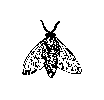
\epsfig{file=fly.eps}
%~ \caption{A sample black and white graphic (.eps format).}
%~ \end{figure}
%~
%~ \begin{figure}
%~ \centering
%~ 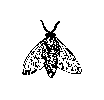
\epsfig{file=fly.eps, height=1in, width=1in}
%~ \caption{A sample black and white graphic (.eps format)
%~ that has been resized with the \texttt{epsfig} command.}
%~ \end{figure}
%~
%~
%~ As was the case with tables, you may want a figure
%~ that spans two columns.  To do this, and still to
%~ ensure proper ``floating'' placement of tables, use the environment
%~ \textbf{figure*} to enclose the figure and its caption.
%~
%~ Note that either {\textbf{.ps}} or {\textbf{.eps}} formats are
%~ used; use
%~ the \texttt{{\char'134}epsfig} or \texttt{{\char'134}psfig}
%~ commands as appropriate for the different file types.
%~
%~ \subsection{Theorem-like Constructs}
%~ Other common constructs that may occur in your article are
%~ the forms for logical constructs like theorems, axioms,
%~ corollaries and proofs.  There are
%~ two forms, one produced by the
%~ command \texttt{{\char'134}newtheorem} and the
%~ other by the command \texttt{{\char'134}newdef}; perhaps
%~ the clearest and easiest way to distinguish them is
%~ to compare the two in the output of this sample document:
%~
%~ This uses the \textbf{theorem} environment, created by
%~ the\linebreak\texttt{{\char'134}newtheorem} command:
%~ \newtheorem{theorem}{Theorem}
%~ \begin{theorem}
%~ Let $f$ be continuous on $[a,b]$.  If $G$ is
%~ an antiderivative for $f$ on $[a,b]$, then
%~ \begin{displaymath}\int^b_af(t)dt = G(b) - G(a).\end{displaymath}
%~ \end{theorem}
%~
%~ The other uses the \textbf{definition} environment, created
%~ by the \texttt{{\char'134}newdef} command:
%~ \newdef{definition}{Definition}
%~ \begin{definition}
%~ If $z$ is irrational, then by $e^z$ we mean the
%~ unique number which has
%~ logarithm $z$: \begin{displaymath}{\log e^z = z}\end{displaymath}
%~ \end{definition}
%~
%~ \begin{figure}
%~ \centering
%~ \psfig{file=rosette.ps, height=1in, width=1in,}
%~ \caption{A sample black and white graphic (.ps format) that has
%~ been resized with the \texttt{psfig} command.}
%~ \end{figure}
%~
%~ Two lists of constructs that use one of these
%~ forms is given in the
%~ \textit{Author's  Guidelines}.
%~
%~ \begin{figure*}
%~ \centering
%~ 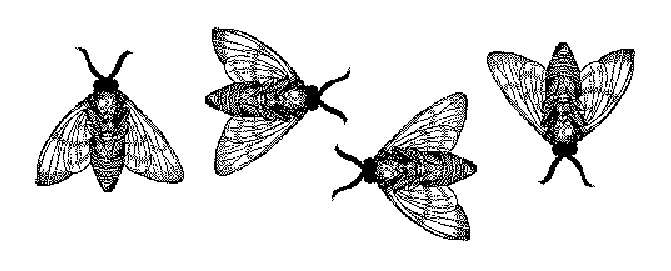
\epsfig{file=flies.eps}
%~ \caption{A sample black and white graphic (.eps format)
%~ that needs to span two columns of text.}
%~ \end{figure*}
%~ and don't forget to end the environment with
%~ {figure*}, not {figure}!
 %~
%~ There is one other similar construct environment, which is
%~ already set up
%~ for you; i.e. you must \textit{not} use
%~ a \texttt{{\char'134}newdef} command to
%~ create it: the \textbf{proof} environment.  Here
%~ is a example of its use:
%~ \begin{proof}
%~ Suppose on the contrary there exists a real number $L$ such that
%~ \begin{displaymath}
%~ \lim_{x\rightarrow\infty} \frac{f(x)}{g(x)} = L.
%~ \end{displaymath}
%~ Then
%~ \begin{displaymath}
%~ l=\lim_{x\rightarrow c} f(x)
%~ = \lim_{x\rightarrow c}
%~ \left[ g{x} \cdot \frac{f(x)}{g(x)} \right ]
%~ = \lim_{x\rightarrow c} g(x) \cdot \lim_{x\rightarrow c}
%~ \frac{f(x)}{g(x)} = 0\cdot L = 0,
%~ \end{displaymath}
%~ which contradicts our assumption that $l\neq 0$.
%~ \end{proof}
%~
%~ Complete rules about using these environments and using the
%~ two different creation commands are in the
%~ \textit{Author's Guide}; please consult it for more
%~ detailed instructions.  If you need to use another construct,
%~ not listed therein, which you want to have the same
%~ formatting as the Theorem
%~ or the Definition\cite{salas:calculus} shown above,
%~ use the \texttt{{\char'134}newtheorem} or the
%~ \texttt{{\char'134}newdef} command,
%~ respectively, to create it.
%~
%~ \subsection*{A {\secit Caveat} for the \TeX\ Expert}
%~ Because you have just been given permission to
%~ use the \texttt{{\char'134}newdef} command to create a
%~ new form, you might think you can
%~ use \TeX's \texttt{{\char'134}def} to create a
%~ new command: \textit{Please refrain from doing this!}
%~ Remember that your \LaTeX\ source code is primarily intended
%~ to create camera-ready copy, but may be converted
%~ to other forms -- e.g. HTML. If you inadvertently omit
%~ some or all of the \texttt{{\char'134}def}s recompilation will
%~ be, to say the least, problematic.

%~ This paragraph will end the body of this sample document.
%~ Remember that you might still have Acknowledgments or
%~ Appendices; brief samples of these
%~ follow.  There is still the Bibliography to deal with; and
%~ we will make a disclaimer about that here: with the exception
%~ of the reference to the \LaTeX\ book, the citations in
%~ this paper are to articles which have nothing to
%~ do with the present subject and are used as
%~ examples only.
%\end{document}  % This is where a 'short' article might terminate

%ACKNOWLEDGMENTS are optional
%~ \section{Acknowledgments}
%~ This section is optional; it is a location for you
%~ to acknowledge grants, funding, editing assistance and
%~ what have you.  In the present case, for example, the
%~ authors would like to thank Gerald Murray of ACM for
%~ his help in codifying this \textit{Author's Guide}
%~ and the \textbf{.cls} and \textbf{.tex} files that it describes.

%
% The following two commands are all you need in the
% initial runs of your .tex file to
% produce the bibliography for the citations in your paper.
\bibliographystyle{abbrv}
%\bibliography{sigproc}  % sigproc.bib is the name of the Bibliography in this case
\begin{thebibliography}{10}

\bibitem{tuw}
\textit{Tell Us Where}.
\newblock http://telluswhere.net.
\newblock Location based mobile game.

\bibitem{Bateman:data}
J.~Bateman, T.~Tenbrink, and S.~Farrar.
\newblock The role of conceptual and linguistic ontologies in interpreting
  spatial discourse.
\newblock {\em Discourse Processes}, 44(3):175--212, 2007.

\bibitem{Bateman:language}
J.~A. Bateman.
\newblock Language and space: A two-level semantic approach based
  on principles of ontological engineering.
\newblock {\em International Journal of Speech Technology}, 13(1):29--48, 2010.

\bibitem{Bateman:ontology}
J.~A. Bateman, J.~Hois, R.~Ross, and T.~Tenbrink.
\newblock A linguistic ontology of space for natural language processing.
\newblock {\em Artificial Intelligence}, 174(14):1027--1071, 2010.

\bibitem{daniel:modes}
M.-P. Daniel, L.~Carite, and M.~Denis.
\newblock Modes of linearization in the description of spatial configurations.
\newblock In J.~Portugali, editor, {\em The Construction of Cognitive Maps},
  volume~32 of {\em GeoJournal Library}, pages 297--318. Kluwer Academic,
  Dordrecht, 1996.

\bibitem{marneffe:stanford}
M.-C. de~Marneffe and C.~D. Manning.
\newblock Stanford typed dependencies manual.
\newblock http://nlp.stanford.edu/software/dependencies\_manual.pdf, 2008.

\bibitem{CLEF:data}
M.~Grubinger, P.~Clough, H.~M{\"u}ller, and T.~Deselaers.
\newblock The {IAPR TC}-12 benchmark: A new evaluation resource for visual
  information systems.
\newblock In {\em Proceedings of the International Workshop OntoImage 2006 --
  Language Resources for Content Based Image Retrieval}, pages 13--23, 2006.

\bibitem{herskovits:pragmatics}
A.~Herskovits.
\newblock Semantics and pragmatics of locative expressions.
\newblock {\em Cognitive Science}, 9(3):341--378, 1985.

\bibitem{kelleher:perceptually}
J.~D. Kelleher.
\newblock {\em A perceptually based computational framework for the
  interpretation of spatial language}.
\newblock PhD thesis, Dublin City University, 2003.

\bibitem{klein:accurate}
D.~Klein and C.~D. Manning.
\newblock Accurate unlexicalized parsing.
\newblock In {\em Proceedings of the 41st Annual Meeting on Association for
  Computational Linguistics-Volume 1}, pages 423--430. Association for
  Computational Linguistics, 2003.

\bibitem{tellex:language}
T.~Kollar, S.~Tellex, D.~Roy, and N.~Roy.
\newblock Toward understanding natural language directions.
\newblock In {\em 5th ACM/IEEE International Conference on Human-Robot
  Interaction}, pages 259--266, 2010.

\bibitem{parisa:semeval}
P.~Kordjamshidi, S.~Bethard, and M.-F. Moens.
\newblock Sem{E}val-2012 {T}ask 3: Spatial role labeling.
\newblock In {\em Proceedings of the {S}em{E}val-2012 Evaluation Exercises}.
  Association for Computational Linguistics, 2012.

\bibitem{kordjamshidi:language}
P.~Kordjamshidi, M.~Van~Otterlo, and M.-F. Moens.
\newblock From language towards formal spatial calculi.
\newblock In {\em Workshop on Computational Models of Spatial Language
  Interpretation (CoSLI 2010)}, 2010.

\bibitem{Kordjamshidi:labelling}
P.~Kordjamshidi, M.~Van~Otterlo, and M.-F. Moens.
\newblock Spatial role labeling: Towards extraction of spatial relations from
  natural language.
\newblock {\em ACM Transactions on Speech and Language Processing},
  8(3):4:1--4:36, 2011.

\bibitem{landau:and}
B.~Landau and R.~Jackendoff.
\newblock ``{W}hat'' and ``where'' in spatial language and spatial cognition.
\newblock {\em Behavioral and Brain Sciences}, 16:217--217, 1993.

\bibitem{Hanjing:route}
H.~Li, T.~Zhao, S.~Li, and J.~Zhao.
\newblock The extraction of trajectories from real texts based on linear
  classification.
\newblock In J.~Nivre, H.-J. Kaalep, K.~Muischnek, and M.~Koit, editors, {\em
  Proceedings of the 16th Nordic Conference of Computational Linguistics
  NODALIDA-2007}, pages 121--127, University of Tartu, Finland, 2007.

\bibitem{linde:spatial}
C.~Linde and W.~Labov.
\newblock Spatial networks as a site for the study of language and thought.
\newblock {\em Language}, 51(4):924--939, 1975.

\bibitem{litkowski:semeval}
K.~Litkowski and O.~Hargraves.
\newblock Sem{E}val-2007 {T}ask 06: Word-sense disambiguation of prepositions.
\newblock In {\em Proceedings of the 4th International Workshop on Semantic
  Evaluations}, pages 24--29. Association for Computational Linguistics, 2007.

\bibitem{fei:locative}
F.~Liu.
\newblock Automatic identification of locative expressions from informal text.
\newblock Master's thesis, University of Melbourne, Australia, 2013.

\bibitem{matuszek:following}
C.~Matuszek, D.~Fox, and K.~Koscher.
\newblock Following directions using statistical machine translation.
\newblock In {\em Proceedings of the 5th ACM/IEEE International Conference on
  Human-Robot Interaction}, pages 251--258. IEEE Press, 2010.

\bibitem{olivier:semantics}
P.~Olivier and J.-i. Tsujii.
\newblock A computational view of the cognitive semantics of spatial
  prepositions.
\newblock In {\em Proceedings of the 32nd Annual Meeting of the Association for
  Computational Linguistics}, pages 303--309. Association for Computational
  Linguistics, 1994.

\bibitem{tappan:knowledge}
D.~A. Tappan.
\newblock {\em Knowledge-based spatial reasoning for automated scene generation
  from text descriptions}.
\newblock PhD thesis, New Mexico State University, Las Cruces, NM, USA, 2004.

\bibitem{igor:annotations}
I.~Tytyk and T.~Baldwin.
\newblock Component-wise annotation and analysis of informal place
  descriptions.
\newblock In M.~Vasardani, S.~Winter, K.-F. Richter, K.~Janowicz, and
  W.~Mackaness, editors, {\em International Workshop on Place-Related Knowledge
  Acquisition Research}, volume 881 of {\em CEUR}, pages 7--12, 2012.

\bibitem{maria:descriptions}
M.~Vasardani, S.~Timpf, S.~Winter, and M.~Tomko.
\newblock From descriptions to depictions: a conceptual framework.
\newblock In {\em Spatial Information Theory}, Lecture Notes in Computer
  Science, Berlin, 2013. Springer.

\bibitem{xu:case}
L.~D. Xu.
\newblock Case based reasoning.
\newblock {\em IEEE Potentials}, 13(5):10--13, 1994.

\bibitem{zlatev:semantics}
J.~Zlatev.
\newblock Spatial semantics.
\newblock {\em Handbook of Cognitive Linguistics}, pages 318--350, 2007.

\end{thebibliography}

%\end{thebibliography}

% You must have a proper ".bib" file
%  and remember to run:
% latex bibtex latex latex
% to resolve all references
%
% ACM needs 'a single self-contained file'!
%
%APPENDICES are optional
%\balancecolumns
%\appendix
%Appendix A
%~ \section{Headings in Appendices}
%~ The rules about hierarchical headings discussed above for
%~ the body of the article are different in the appendices.
%~ In the \textbf{appendix} environment, the command
%~ \textbf{section} is used to
%~ indicate the start of each Appendix, with alphabetic order
%~ designation (i.e. the first is A, the second B, etc.) and
%~ a title (if you include one).  So, if you need
%~ hierarchical structure
%~ \textit{within} an Appendix, start with \textbf{subsection} as the
%~ highest level. Here is an outline of the body of this
%~ document in Appendix-appropriate form:
%~ \subsection{Introduction}
%~ \subsection{The Body of the Paper}
%~ \subsubsection{Type Changes and  Special Characters}
%~ \subsubsection{Math Equations}
%~ \paragraph{Inline (In-text) Equations}
%~ \paragraph{Display Equations}
%~ \subsubsection{Citations}
%~ \subsubsection{Tables}
%~ \subsubsection{Figures}
%~ \subsubsection{Theorem-like Constructs}
%~ \subsubsection*{A Caveat for the \TeX\ Expert}
%~ \subsection{Conclusions}
%~ \subsection{Acknowledgments}
%~ \subsection{Additional Authors}
%~ This section is inserted by \LaTeX; you do not insert it.
%~ You just add the names and information in the
%~ \texttt{{\char'134}additionalauthors} command at the start
%~ of the document.
%~\subsection{References}
%~Generated by bibtex from your ~.bib file.  Run latex,
%~then bibtex, then latex twice (to resolve references)
%~to create the ~.bbl file.  Insert that ~.bbl file into
%~the .tex source file and comment out
%~the command \texttt{{\char'134}thebibliography}.
% This next section command marks the start of
% Appendix B, and does not continue the present hierarchy
%\section{More Help for the Hardy}
%The acm\_proc\_article-sp document class file itself is chock-full of succinct
%and helpful comments.  If you consider yourself a moderately
%experienced to expert user of \LaTeX, you may find reading
%it useful but please remember not to change it.
\balancecolumns
% That's all folks!
\end{document}
